
\begin{center}
	\Huge
	Dobbeltpunkter
\end{center}

\section*{Dobbeltpunkter for vektorfunktioner}
\stepcounter{section}

Vi har set flere eksempler på vektorfunktioner hvis parameterkurver skærer gennem sig selv. Et sådant punkt, hvor dette forekommer kalder vi et dobbeltpunkt, og vi skal se, hvordan vi finder disse punkter. 

\begin{exa}
	Lad os betragte vektorfunktionen $\vv{r}$ givet ved
	\begin{align*}
		\vv{r}(t) = 
		\begin{pmatrix}
			t^3-4t \\
			t^2
		\end{pmatrix}.
	\end{align*}
	Vi får at vide, at vektorfunktionen har et dobbeltpunkt, når $t=2$. Vi ønsker at bestemme den anden værdi for $t$, så vi også rammer dette punkt. 
	Vi starter med at finde punktet.
	\begin{align*}
		\vv{r}(2) = 
		\begin{pmatrix}
			2^3-4\cdot 2 \\
			2^2
		\end{pmatrix} =
		\begin{pmatrix}
			0 \\
			4
		\end{pmatrix}.
	\end{align*}
	Vi skal derfor bestemme $t$, så vektorfunktionen rammer punktet $P_t(0,4)$. Vi betragter derfor ligningen
	\begin{align*}
		t^2 = 4, 
	\end{align*}
	og får at den anden løsning må være $t=-2$. Dette indsættes for at verificere, og vi får
	\begin{align*}
		\vv{r}(-2) = 
		\begin{pmatrix}
			(-2)^2 - 4(-2) \\
			(-2)^2
		\end{pmatrix} = 
		\begin{pmatrix}
		 	0 \\
		 	4
		\end{pmatrix},
	\end{align*}
	og vi ved derfor, at vi har fundet det rigtige $t$. 
\end{exa}
\begin{exa}
	Vi ønsker at finde dobbeltpunkter for vektorfunktionen $\vv{r}$ givet ved
	\begin{align*}
		\vv{r}(t) =
		\begin{pmatrix}
			t^2-2t \\
			t^4-4t^2
		\end{pmatrix}.
	\end{align*}
	Vi starter med at tegne parameterkurven for $\vv{r}$. Dette gøres ved at skrive følgende i Maple.
	\begin{align*}
		&\texttt{with(Gym):}\\
		&\texttt{r(t):=<t\string^2-2t,t\string^4-4t\string^2>}\\
		&\texttt{vektorPlot(r(t),t=-2..3)}
	\end{align*}
	Vi får så plottet, der kan ses på Fig. \ref{fig:dobbelt}.
	\begin{figure}[H]
		\centering
		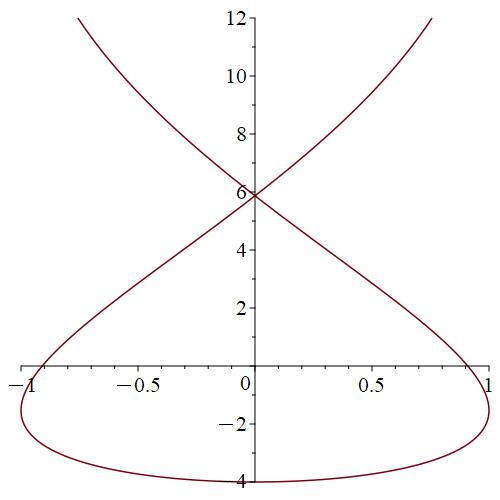
\includegraphics[width=0.7\textwidth]{Billeder/dobbeltpunkt.jpg}
		\caption{Parameterkurve for vektorfunktion med dobbeltpunkt}
		\label{fig:dobbelt}
	\end{figure}
	Det ser ud til at der er et dobbeltpunkt i $(0,0)$. Vi afgør dette ved at indføre en ny vektorfunktion $\vv{v}$ givet ved
	\begin{align*}
		\vv{v}(t) =
		\begin{pmatrix}
			s^2-2s \\
			s^4-4s^2
		\end{pmatrix}.
	\end{align*}
	Denne vektorfunktion er i princippet lig $\vv{r}$, men nu med en ny parameter $s$. Vi skal løse ligningen
	\begin{align*}
		 \vv{r}(t) = \vv{v}(s). 
	\end{align*}
	Dette gøres i Maple ved at skrive følgende. 
	\begin{align*}
		\texttt{solve([t\string^2-2t=s\string^2-2s,t\string^4-4t\string^2=s\string^4-4s\string^2])}
	\end{align*}
	Dette giver os løsningen $t= 2, s=0$, så dobbeltpunktet findes altså når $t=0$ eller når $t=2$. Dette indsættes i $\vv{r}$ og vi får
	\begin{align*}
		\vv{r}(0) = 
		\begin{pmatrix}
			0 \\ 0
		\end{pmatrix},
	\end{align*}
	og dobbeltpunktet er altså i $(0,0)$ som forventet. 
	Vi vil gerne bestemme vinklen mellem tangenterne i dobbeltpunktet. Vi bestemmer derfor tangentvektorerne:
	\begin{align*}
		\vv{r}'(2) = 
		\begin{pmatrix}
			2\cdot 2-2 \\
			4\cdot 2^3-8\cdot 2
		\end{pmatrix} =
		\begin{pmatrix}
			2 \\
			16
		\end{pmatrix}
	\end{align*}
	Tilsvarende gøres for $t=0$.
	\begin{align*}
		\vv{r}'(0) = 
		\begin{pmatrix}
			2\cdot 0 - 2 \\
			4\cdot 0^3-8\cdot 0
		\end{pmatrix} =
		\begin{pmatrix}
			-2 \\
			0
		\end{pmatrix}
	\end{align*}
	Vi bestemmer vinklen mellem disse i Maple og får vinklen til at være $97.1^\circ$.
\end{exa}

\section*{Opgave 1 (Uden Maple)}

\begin{enumerate}[label=\roman*)]
	\item En vektorfunktion $\vv{r}$ er givet ved
	\begin{align*}
		\vv{r}(t) = 
		\begin{pmatrix}
			t^2 \\
			t^3-8t
		\end{pmatrix}.
	\end{align*}
	Den har et dobbeltpunkt, når $t=-4$. Bestem det andet $t$, så $\vv{r}$ rammer dette punkt
\end{enumerate}
\section*{Opgave 2 (Med Maple)}
\begin{enumerate}[label=\roman*)]
	\item En vektorfunktion $\vv{r}$ er givet ved
	\begin{align*}
		\vv{r}(t) = 
		\begin{pmatrix}
			\sin(t) \\
			t^2-4
		\end{pmatrix}.
	\end{align*}
	Parameterkurven for $\vv{r}$ har et dobbeltpunkt, når $t=\pi$. Bestem den anden værdi for $t$, der tilsvarer dette punkt. 
	\item En vektorfunktion $\vv{r}$ er givet ved
	\begin{align*}
		\vv{r}(t) = 
		\begin{pmatrix}
			\sin(t) \\
			t^2-4
		\end{pmatrix}.
	\end{align*}
	Parameterkurven for $\vv{r}$ har et dobbeltpunkt, når $t=\pi$. Bestem den anden værdi for $t$, der tilsvarer dette punkt. 
	\item En vektorfunktion $\vv{r}$ er givet ved
	\begin{align*}
		\vv{r}(t) = 
		\begin{pmatrix}
			t^3-3t^2-t+3 \\
			t^4-4t^3+t^2+8t-6
		\end{pmatrix}.
	\end{align*}
	Parameterkurven for $\vv{r}$ har et dobbeltpunkt, når $t=1$. Bestem den anden værdi for $t$, og bestem vinklen mellem tangentvektorerne i dette punkt. 
\end{enumerate}


\section*{Opgave 3}

\begin{enumerate}[label=\roman*)]
	\item En vektorfunktion er givet ved
	\begin{align*}
		\vv{r}(t) = 
		\begin{pmatrix}
			t^3-6t,t^2-5
		\end{pmatrix}.
	\end{align*}
	Tegn først $\vv{r}$ og bestem derefter eventuelle dobbeltpunkter for $\vv{r}$.
	\item En vektorfunktion er givet ved
	\begin{align*}
		\vv{r}(t) = 
		\begin{pmatrix}
			\cos(t)+\sin(t),t^2-4
		\end{pmatrix}.
	\end{align*}
	Tegn først $\vv{r}$ og bestem derefter eventuelle dobbeltpunkter for $\vv{r}$, \\ når $-5<t<5$. Bestem desuden vinklen mellem tangentvektorerne i dette punkt.
\end{enumerate}
